Wie auch im Abschnitt \ref{sec:ergebnisseSichtpruefungDurchLichtstreuung} soll das Verfahren zunächst mit der Durchlichtauswertung auf transparente Prüfobjekte angewandt werden.
Für einen nachfolgenden Vergleich zum Verfahren \glqq Sichtprüfung durch Lichtstreuung\grqq ~sollen mit diesem Verfahren auch die Brillengläser 1 und 2 aus Abbildung \ref{tikz:abbStreifenaufnahmen} ausgewertet werden.
Zusätzlich zu den beiden Objekten wird ein weiteres Brillenglas mit diesem Verfahren untersucht.
Es wird der Aufbau aus dem linken Teilbild aus Abbildung \ref{tikz:abbAufbauFotos} verwendet und die Brillengläser auf die dunkle Halterung positioniert.
Die Brillengläser werden zur Demonstration bei der Anzeige eines einzelnen Streifenmusters nach den Parametern aus Tabelle \ref{tab:paramDeflektometrischRegistrierung} aufgenommen:

% Abbildung: Aufnahmen mit sinusoidalen Streifenmustern
{
	\begin{figure}[H]
		\centering
		\begin{adjustbox}{width=\textwidth}
	\begin{tikzpicture}[every node/.style={inner sep=0,outer sep=0}]
		% Bilder
		\node [anchor=north west] (img1) at (0,0) {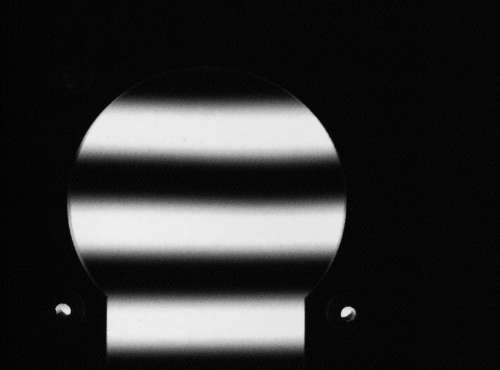
\includegraphics[width=.31\textwidth]{05_ergebnisse/ergDeflektometrischeRegistrierung/durchlichtAuswertungDeflektometrischeRegistrierung/figures/brillenglas_1_streifenmuster}};
		
		\node [anchor=north west] (img2) at (0.345\textwidth,0) {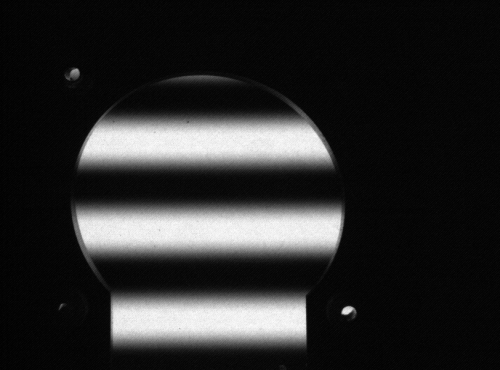
\includegraphics[width=.31\textwidth]{05_ergebnisse/ergDeflektometrischeRegistrierung/durchlichtAuswertungDeflektometrischeRegistrierung/figures/brillenglas_2_streifenmuster}};
		
		\node [anchor=north west] (img3) at (0.69\textwidth,0) {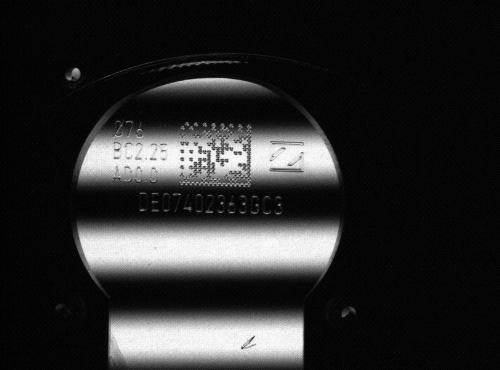
\includegraphics[width=.31\textwidth]{05_ergebnisse/ergDeflektometrischeRegistrierung/durchlichtAuswertungDeflektometrischeRegistrierung/figures/brillenglas_4_streifenmuster}};
		
		% Captions
		\node [below=0.2cm of img1] (cap1) {Brillenglas 1};
		\node [below=0.2cm of img2] (cap2) {Brillenglas 2};
		\node [below=0.2cm of img3] (cap3) {Brillenglas 4};			
	\end{tikzpicture}
\end{adjustbox}
\caption[Aufnahmen der Brillengläser bei der Durchlichtauswertung mit sinusoidalen Streifenmustern]{Aufnahmen der Brillengläser bei der Durchlichtauswertung mit sinusoidalen Streifenmustern}
		\label{tikz:abbSinusStreifenaufnahmen}
	\end{figure}
}

\noindent
Nach der Bestimmung der deflektometrischen Registrierungen der Brillengläser können daraus Bilder erstellt werden (siehe Definition \ref{def:graphDeflektometrischeRegistrierung}):

% Abbildung: Bilder der deflektometrische Registrierung der Zeilen
{
	\begin{figure}[H]
		\begin{adjustbox}{width=\textwidth}
	\begin{tikzpicture}[every node/.style={inner sep=0,outer sep=0}]
		% Bilder
		\node [anchor=north west] (img1) at (0,0) {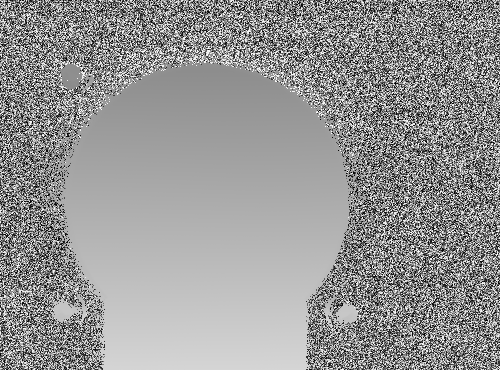
\includegraphics[width=.31\textwidth]{05_ergebnisse/ergDeflektometrischeRegistrierung/durchlichtAuswertungDeflektometrischeRegistrierung/figures/brillenglas_1_registrierung}};
		
		\node [anchor=north west] (img2) at (0.345\textwidth,0) {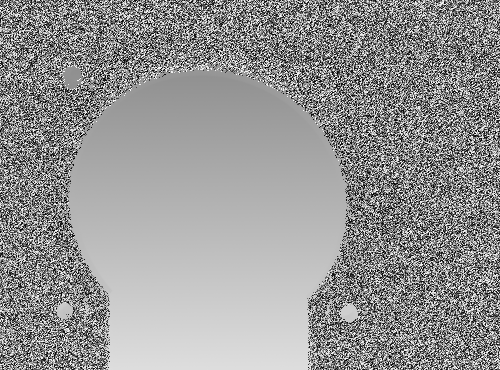
\includegraphics[width=.31\textwidth]{05_ergebnisse/ergDeflektometrischeRegistrierung/durchlichtAuswertungDeflektometrischeRegistrierung/figures/brillenglas_2_registrierung}};
		
		\node [anchor=north west] (img3) at (0.69\textwidth,0) {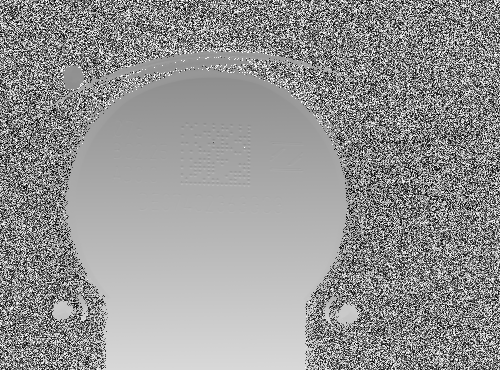
\includegraphics[width=.31\textwidth]{05_ergebnisse/ergDeflektometrischeRegistrierung/durchlichtAuswertungDeflektometrischeRegistrierung/figures/brillenglas_4_registrierung}};
		
		% Captions
		\node [below=0.2cm of img1] (cap1) {Brillenglas 1};
		\node [below=0.2cm of img2] (cap2) {Brillenglas 2};
		\node [below=0.2cm of img3] (cap3) {Brillenglas 4};			
	\end{tikzpicture}
\end{adjustbox}
\caption[Bilder der deflektometrischen Registrierung der Zeilen bei der Durchlichtauswertung]{Bilder der deflektometrischen Registrierung der Zeilen bei der Durchlichtauswertung.}
		\label{tikz:abbDeflectometricRegistrations}
	\end{figure}
}

\noindent
Zur Verdeutlichung der Ergebnisse des Verfahrens ist es sinnvoll, die Ableitung der Bilder in Richtung der Zeilen zu bilden (siehe Abschnitt \ref{sec:auswertungDeflektometrischeRegistrierung}).
Nach einer Kontrastverbesserung innerhalb des Objekts erhält man folgende Bilder:

% Abbildung: Bilder der Ableitung der deflektometrische Registrierung der Zeilen
{
	\begin{figure}[H]
		\centering
		\begin{adjustbox}{width=\textwidth}
	\begin{tikzpicture}[every node/.style={inner sep=0,outer sep=0}]
		% Bilder
		\node [anchor=north west] (img1) at (0,0) {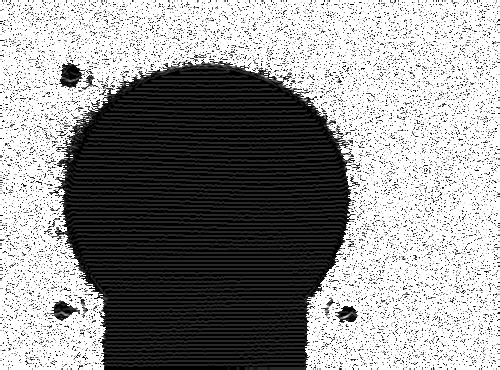
\includegraphics[width=.31\textwidth]{05_ergebnisse/ergDeflektometrischeRegistrierung/durchlichtAuswertungDeflektometrischeRegistrierung/figures/brillenglas_1_ableitung}};
		
		\node [anchor=north west] (img2) at (0.345\textwidth,0) {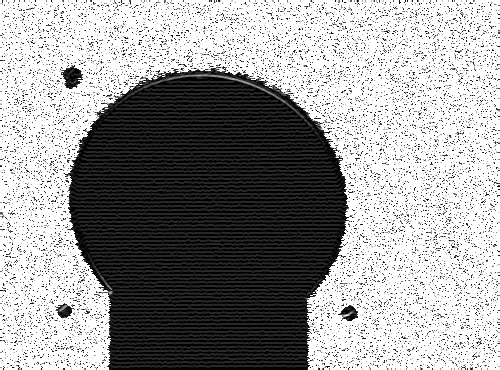
\includegraphics[width=.31\textwidth]{05_ergebnisse/ergDeflektometrischeRegistrierung/durchlichtAuswertungDeflektometrischeRegistrierung/figures/brillenglas_2_ableitung}};
		
		\node [anchor=north west] (img3) at (0.69\textwidth,0) {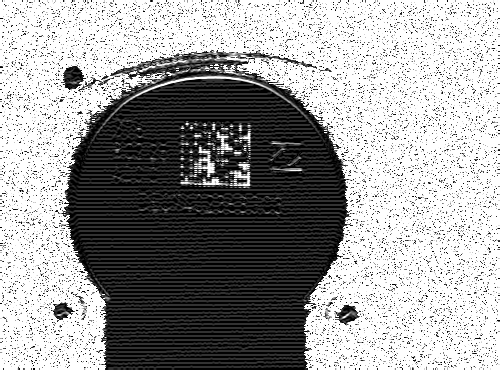
\includegraphics[width=.31\textwidth]{05_ergebnisse/ergDeflektometrischeRegistrierung/durchlichtAuswertungDeflektometrischeRegistrierung/figures/brillenglas_4_ableitung}};
		
		% Captions
		\node [below=0.2cm of img1] (cap1) {Brillenglas 1};
		\node [below=0.2cm of img2] (cap2) {Brillenglas 2};
		\node [below=0.2cm of img3] (cap3) {Brillenglas 4};			
	\end{tikzpicture}
\end{adjustbox}
\caption[Ableitung der deflektometrischen Registrierung der Zeilen bei der Durchlichtauswertung]{Ableitung der deflektometrischen Registrierung der Zeilen bei der Durchlichtauswertung.}
		\label{tikz:abbAbleitungRegistrierungDurchlicht}
	\end{figure}
}

\noindent
Für die Brillengläser 1 und 2 lassen sich in Abbildung \ref{tikz:abbAbleitungRegistrierungDurchlicht} keine auffällige Stellen entdecken, obwohl Kratzer und Gravuren vorhanden sind (vgl. Abbildung \ref{tikz:abbNachbearbeitung}).
Für alle Brillengläser erkennt man aber horizontale hellere Streifen in den Ableitungsbildern.
Diese entstehen durch die gleichmäßige Krümmung der Brillengläser in Richtung der Zeilen.
Man erfasst durch die Anwendung der deflektometrischen Zeilenregistrierung besonders die Krüm\-mungs\-ab\-wei\-chun\-gen in der Zeilenrichtung.
Deshalb werden die horizontalen Krüm\-mungs\-ab\-wei\-chun\-gen deutlicher.
Im Ableitungsbild von Brillenglas 3 in Abbildung \ref{tikz:abbAbleitungRegistrierungDurchlicht} sind Auffälligkeiten erkennbar.
Dabei sieht man das eingravierte Markenkennzeichen und einen Data-Matrix-Code zur Codierung von Informationen für den Brillenglashersteller.